%!TEX root =  main.tex

\lectureheader{162}{Calculus II}{Calculus on parametric equations}{\textit{Thomas' Calculus} \textsection 11.2}

\begin{theorem}
If $x$ and $y$ are given as functions of the parameter $t$, then
\begin{equation*}
\frac{\dee y}{\dee x} = \frac{\frac{\dee y}{\dee t}}{\frac{\dee x}{\dee t}}
\end{equation*}
whenever $\frac{\dee x}{\dee t}\ne 0$.
\end{theorem}

\begin{example}
Find the tangent line to the curve
\begin{align*}
x &= \sec t,\\
y &= \tan t
\end{align*}
at the point $(\sqrt 2, 1)$, i.e., when $t=\pi/4$.
\end{example}

\newpage

\begin{example}
Compute $\frac{\dee^2 y}{\dee x^2}$ as a function of $t$ is
\begin{align*}
x & = t-t^2,\\
y &= t-t^3.
\end{align*}
\end{example}

\newpage

\begin{remark}\,
\begin{itemize}
\item The substitution rule (i.e., chain rule in reverse) can help us compute areas in parametric form as well.
\item If $y$ is a function of $x$ and $x$ is a function of $t$, then
\begin{equation*}
\int_{x(a)}^{x(b)}y\dee x = \int_a^b y(t)\frac{\dee x}{\dee t}\dee t.
\end{equation*}
\end{itemize}
\end{remark}

\begin{example}
Find the area enclosed by the astroid
\begin{align*}
x &= \cos^3 t,\\
y &= \sin^3 t\quad (0\le t\le 2\pi).
\end{align*}
\begin{flushright}
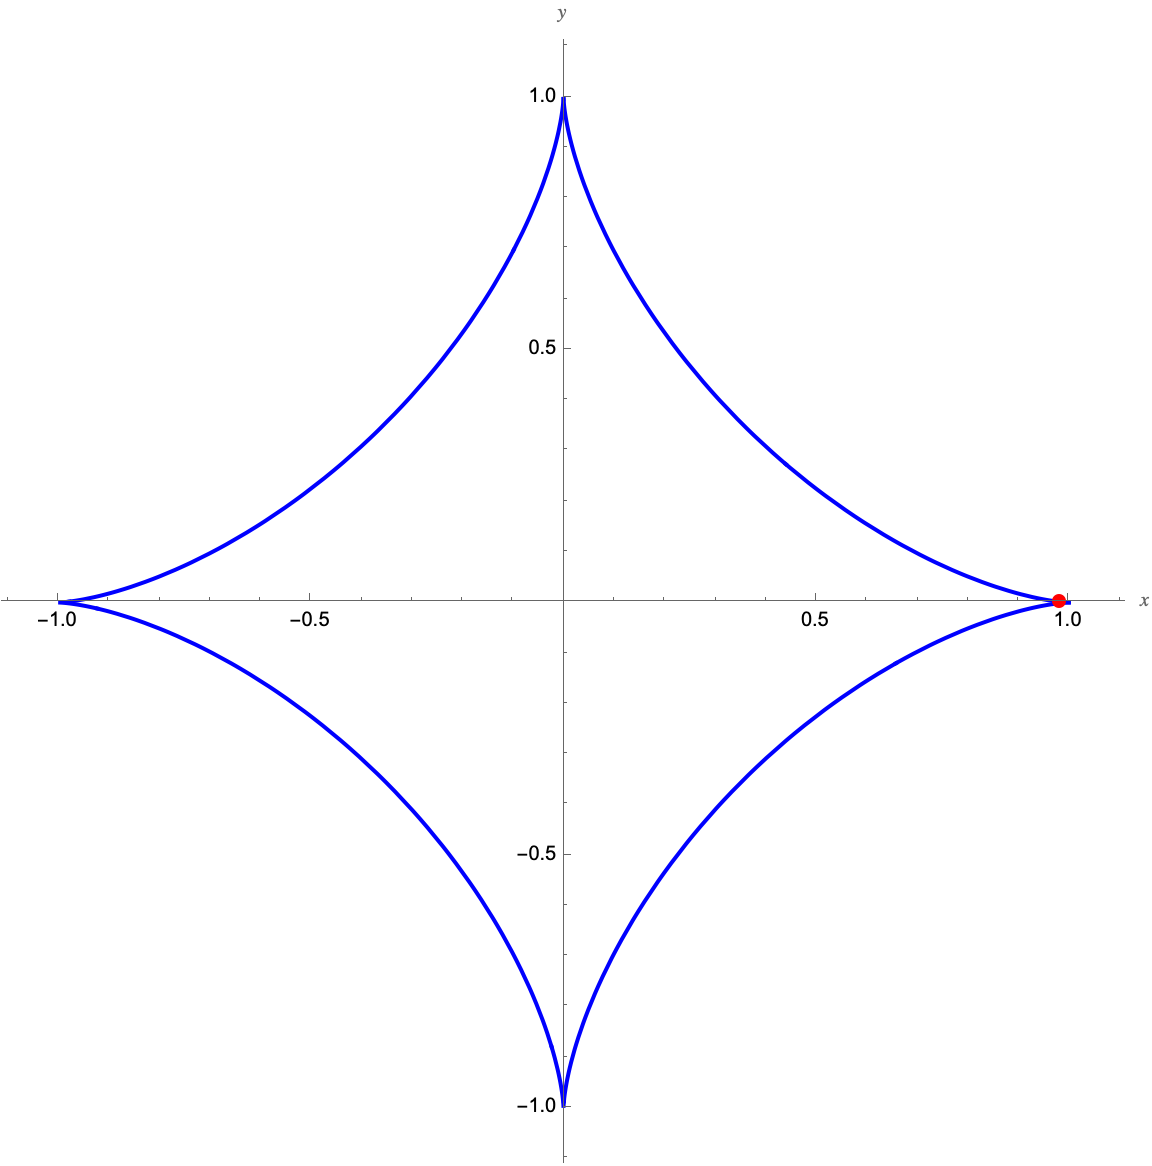
\includegraphics[width=2.5in]{img/astroid}
\end{flushright}
\end{example}

\newpage

\begin{definition}
Given a parametric curve $C$ that is traversed exactly once as $t$ varies from $\alpha$ to $\beta$, we define the \textbf{arc length differential} by
\begin{equation*}
\dee s = \sqrt{\dee x^2 + \dee y^2},
\end{equation*}
and we define the \textbf{arc length} of $C$ by
\begin{equation*}
s = \int_C\dee s = \int_\alpha^\beta\sqrt{\left(\frac{\dee x}{\dee t}\right)^2 + \left(\frac{\dee y}{\dee t}\right)^2}\dee t
\end{equation*}
provided that the integral exists.
\end{definition}

\begin{remark}\,
\begin{itemize}
\item It is tradition to denote arc length by $s$ for the Latin \textit{spatium}.
\item The definition of $\dee s$ is based on the distance formula and is meant to signify an ``infinitesimal" distance traveled \textit{along} the curve $C$.  
\item In particular, if $C$ passes through the points $(x_{i-1}, y_{i-1})$ and $(x_i, y_i)$, then then distance $\Delta s_i$ traveled \textit{along} $C$ between these two points may be approximated by the straight line distance between the two points, i.e.,
\begin{equation*}
\Delta s_i \approx \sqrt{\Delta x_i^2 + \Delta y_i^2},
\end{equation*}
where $\Delta x_i = x_i-x_{i-1}$ and $\Delta y_i = y_i - y_{i-1}$.
\item Observe that $\dee s$ has the correct units of length attached to it.
\end{itemize}
\end{remark}

\begin{example}
Compute the length of the astroid
\begin{align*}
x &= \cos^3 t,\\
y &= \sin^3 t\quad (0\le t\le 2\pi).
\end{align*}
\end{example}

\newpage



\begin{definition}
Suppose that the parametric curve $C$ is traversed exactly once as $t$ varies from $\alpha$ to $\beta$.
If $C$ is rotated about the $x$-axis to generate a surface of revolution $S$, we define the \textbf{(surface) area} $A$ of the resulting \textit{surface of revolution} by
\begin{equation*}
A = \int_C 2\pi y\dee s =2\pi \int_\alpha^\beta y(t)\sqrt{\left(\frac{\dee x}{\dee t}\right)^2 + \left(\frac{\dee y}{\dee t}\right)^2}\dee t
\end{equation*}
provided that the integral exists.
\end{definition}

\begin{remark}\,
\begin{itemize}
\item If $C$ is rotated about the $y$-axis, then 
\begin{equation*}
A = \int_C 2\pi x\dee s =2\pi \int_\alpha^\beta x(t)\sqrt{\left(\frac{\dee x}{\dee t}\right)^2 + \left(\frac{\dee y}{\dee t}\right)^2}\dee t.
\end{equation*}
\item The definition is based off the area of the \textit{frustum} of a cone.
\item Observe that, in either case, $A$ has the correct dimensionality.
\end{itemize}
\end{remark}

\begin{example}
Calculate the area of the surface that is generated by rotating the curve $y=\sqrt{4-x^2}$ for $-1\le x\le 1$ about the $x$-axis.
\end{example}

\newpage

\begin{example}
Show that Gabriel's horn has infinite surface area despite having finite volume.
\end{example}

